\newpage
\section{Modellazione Heterogeneous Platform}

La piattaforma eterogenea contiene componenti scritti con diversi formalismi e connessi tutti insieme. Essi sono:
\begin{itemize}
    \item controller, non più implementato con AMS ma come TLM (scelto modello untimed per semplicità;
    \item valvola, in AMS-TDF;
    \item serbatoio, in AMS-LSF internamente e AMS-TDF come interfaccia esterna;
    \item decrifratore XTEA, implementato in RTL.
\end{itemize}
Sono necessari ulteriori componenti "collante":
\begin{itemize}
    \item transattore che permette al sistema valvola-serbatoio di interfacciarsi con l'esterno tramite TLM;
    \item interfaccia RTL alla valvola, obbligatoria perchè TLM non riesce a comunicare direttamente con AMS;
    \item interfaccia RTL al serbatoio;
    \item transattore che collega controller, decifratore e sistema valvola-serbatoio; esso passa le richieste del controllore al resto del sistema, eventualmente decriptate.
\end{itemize}

\begin{figure}[htbp]
    \centering
    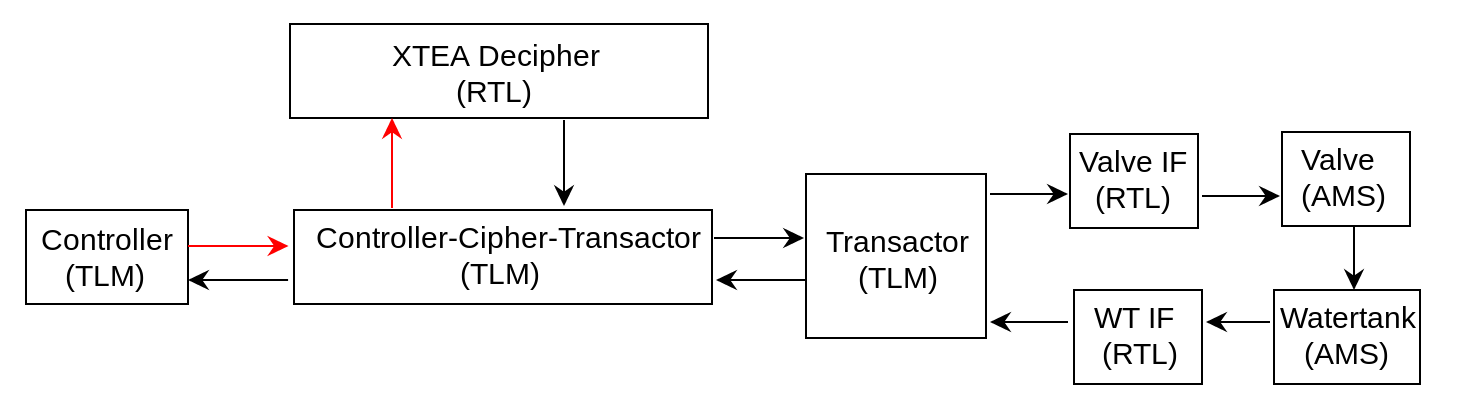
\includegraphics[width=0.5\textwidth]{schemi/het-schema.png}
    \caption{Schema della piattaforma eterogenea. Le freccie in rosso rappresentano il flusso di dati criptato.}
    \label{fig:heterog-platform}
\end{figure}

Lo schema del sistema può essere visto in Figura~\ref{fig:heterog-platform}. Ci sono due flussi di transazioni:
\begin{itemize}
    \item da \code{controller} al \code{controller-cipher-transactor};
    \item da \code{controller-cipher-transactor} a \code{transactor}.
\end{itemize}
Nel primo caso l'initiator è \code{controller}. Se la transazione è in scrittura allora questa conterrà i valori di threshold ed il comando per la valvola. I valori saranno criptati. Il target interroga il decifratore, ed una volta finita l'operazione crea una nuova transazione (secondo flusso). Non vengono ritornati valori all'initiator eccetto l'esito. Se la transazione è in lettura il target porterà avanti la richiesta con una transazione del secondo flusso. Il risultato viene ritornato all'initiator. In questo caso il decifratore non viene usato.

Nel secondo caso l'initiator è \code{controller-cipher -transactor} ed il target è il sistema valvola-serbatoio. Se la transazione è in scrittura allora passo i dati del payload alla valvola, altrimenti leggo i dati del serbatoio. 